\section{Software Development Process}

In order to have a working application at all times, Agile Development was followed.
Unlike typical Agile sprints however, which last one to four weeks, the project was done as one large sprint spanning the entire time.
At the beginning of the project, the task was broken down into two main epics.
These epics were the renderer and the GUI.
The renderer epic was then broken down into smaller user stories, depicting it's entire functionality.
Likewise, the GUI epic was also broken down into user stories outlining how the user would interact with the application.
\\\\
With all the tasks planned out and added to the backlog, they were prioritised and selected for development.
Unlike a normal project, where you would only choose enough stories to fit your capacity, all stories were selected as the project would be completed in one sprint.
It was important during the project to have the application in a working state at all times, iterating on that as the project progressed.
\\\\
This is visible in the way stories were prioritised and the order in which they were completed.
For example, as the key function of the application was to draw images based on ``VEC'' files, the renderer was the first component to be developed.
After this, was the canvas - Which could show the shapes depicted by the actions.
Next the application was iterated upon by adding the different types of actions.
Finally, the ability for the user to interact with the canvas and draw shapes was added.
\\\\
By using this Agile framework, the application was in a usable state, that was better than the last after every iteration.
\begin{center}\fbox{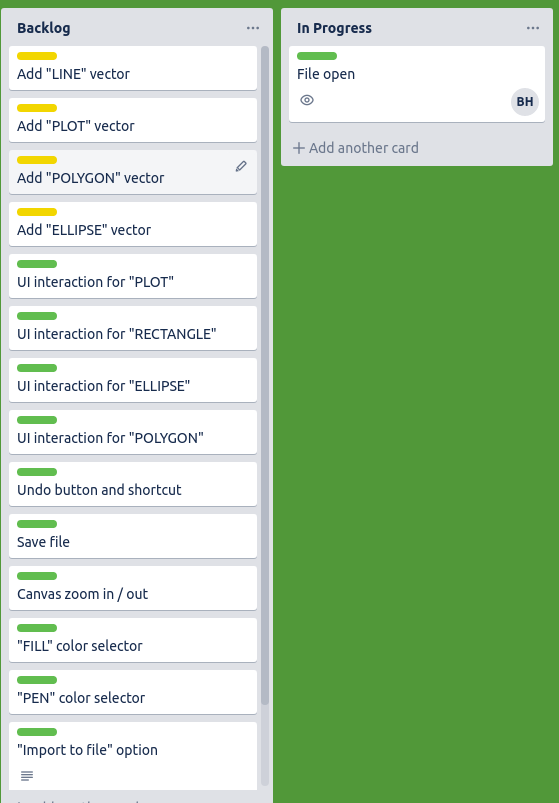
\includegraphics[width=0.6\textwidth]{./images/scrum-board.png}}\end{center}
